\chapter{RELATED WORK}
\label{ch:related-work}

\sepfootnotecontent{fn:speedrun-com-re4-guides}{Footnote: Speedrun.com Resident Evil 4 Guides}

\sepfootnotecontent{fn:beat-em-up}{Footnote: What are beat 'em up games}

In this chapter, we perform a review of previous research and literature related to adaptive systems and dynamic difficulty. We begin by reviewing literature regarding player experience and the concepts that define game difficulty to understand the impact of difficulty in player experience. We attempt to understand how difficulty can be detrimental or a support tool for players to learn, understand and improve upon the use of game mechanics and systems. We identify the problems with fixed difficulty curves, where the game provides a limited set of options for players to define their expected challenge level within the experience of a game. 

We proceed by studying some of the previous solutions that were develop to address the issue of player skill that is not properly represented by a limited set of difficulty curves and challenge levels. First, we understand the concept of player models, where player behavior is monitored and used as a tool to identify game design issues and improvements that directly affect player engagement. We compare that to the recent increase in research towards game analytics, where data from large user bases is aggregated to identify trends, problems and improvement opportunities in regards to game design.

We review some of the pioneering research on AGS (Adaptive Game Systems) \cite{ARTICLE_PlayerCentredGameDesign}, the category of solutions that propose to enhance user experience based on player profile and preferences. We attempt to understand how AGS can be used to alleviate the steep learning curve of highly challenging games, accommodating the skill level of beginner players to the level of challenge proposed by game developers in challenging video games. We review multiple dynamic difficulty implementation methods, such as \emph{probability-based}, \emph{affect-based} and \emph{learning-based} adjustments. We identify the problems with such methods in regards to how these methods can be adapted to commercial solutions, where changes, short deadlines and fast iterations are prevalent.

We also evaluate some of the efforts in adaptivity in commercial games, analyzing their positive and negative effects. We attempt to understand the impact of solutions implemented in some of the most successful commercial games in the last decades, specifying how the discovery of such adaptive systems affected the way that players form strategies and execute actions in such games. We attempt to identify some of the most representative examples in each dynamic adaptation category, and verify the shortcomings of each adaptation method.

% ================================================================================
% ================================================================================
% PLAYER EXPERIENCE AND DIFFICULTY
% ================================================================================
% ================================================================================

\section{Research on Player Experience and Difficulty}

The objective of this work is to create a reliable system that is able to improve experience for any player, regardless of their skill level and expected challenge towards a game. To understand how to improve player experience, we must first define what constitutes it. In this section, we identify the components that constitute player experience based on previous research in usability applied to the specific context of games. 

We attempt to extract concrete, functional features from the subjective term \emph{experience}, and translate these features into tools to design a proper challenge for the player, as well as to avoid mistakes and misconceptions on level design. To perform such a task, we analyze the impact of difficulty in games and its boundaries by reviewing literature on the psychology of player enjoyment. We review why the correct level of challenge can contribute to increasing levels of immersion and the overall positive experience of a player.

\subsection{Definition of Player Experience}

Computer software is commonly developed with the objective of allowing an user to execute a set of tasks, determined by a clear objective and in a specific context \cite{ARTICLE_FromUsabilityToPlayability}. One of the early endeavors in the field of HCI (Human-Computer Interaction) was the efficiency of performing the \emph{task} to ensure a product's instrumental value \cite{ARTICLE_UserExperienceAResearchAgenda}. In this line of thought, users of an application should ideally perform tasks without thinking about the application. 

Research on the interaction between people and systems in the field of HCI led to the concept of \emph{usability}, defined by \cite{ISO_ISO92411} as:

\begin{quotation}
"The extent to which a system, product or service can be used by specified users to achieve specified goals with effectiveness, efficiency and satisfaction in a specified context of use."
\end{quotation}

This definition specifies the three qualities of a usable product: \emph{effectiveness}, \emph{efficiency} and \emph{satisfaction}. We argue that while effectiveness and efficiency can be related to productivity,  satisfaction may not be fulfilled solely by productivity. For instance, an user might feel dissatisfied with the audiovisual components of an application such as its interface, even though the application perfectly satisfies the purpose of assisting in the completion of tasks efficiently.

In \citep{ARTICLE_UserExperienceAResearchAgenda}, we learn that early works on usability expressed that productivity is not primary, but only a contributor to \emph{User Experience}. The term "user experience" does not have a standard definition, but can be seen as how people interact with products and the resulting experience and emotions \cite{ARTICLE_UnderstandingExperience}. The experience is therefore a consequence of: the user's state, such as their emotions and needs; the characteristics of the product, such as usability and audiovisual aspects and the context of use, such as the environment and date.

According to \cite{ARTICLE_FromUsabilityToPlayability}, the concept of \emph{usability} is not sufficient to fully describe UX (User Experience) in relation to Video Games. The authors argue that video games are a specific type of interactive system used for leisure purposes. Thus, when evaluating quality not only instrumental values should be considered, but also non-instrumental values such as storytelling, visuals and character design. The author also introduces the concept of \emph{Player Experience}, a specialization of UX that emphasizes the specific properties of experience in games.

The author explains that Player Experience is characterized by \emph{Playability}, a concept based on Usability but with different meanings in the video game context. The proposed definition of \emph{Playability} by \cite{ARTICLE_FromUsabilityToPlayability} resembles the original Usability definition, but emphasizes the user-centric perspective and the satisfaction property:

\begin{quotation}
"Playability represents the degree to which specified users can achieve specified goals with effectiveness, efficiency and specially satisfaction and fun in a playable context of use."
\end{quotation}

This definition is further explained when the author introduces a set of seven attributes that compose Playability: \emph{Satisfaction}, \emph{Learnability}, \emph{Effectiveness}, \emph{Immersion}, \emph{Motivation}, \emph{Emotion} and \emph{Socialization}. The concepts of effectiveness and satisfaction remain present in this definition, but are specialized or complemented. Efficiency is specified as \emph{learnability} and \emph{immersion}, and the satisfaction aspect is complemented by\emph{emotion}, \emph{motivation} and \emph{socialization} to define a set of user-centred attributes. Since this work focuses on a single-player environment, we will discuss the first six attributes and evaluate which of them can be manipulated by a reliable system through AGT.

\emph{Satisfaction} is the degree of enjoyment derived from playing, characterized by \emph{fun}, \emph{disappointment} and \emph{attractiveness}. Fun is classified as the ability of a game to entertain the player whether through challenge, curiosity or competition. Disappointment refers to the feeling of disappointment of the player in relation to a game. Attractiveness encompasses any functional or aesthetic features that increases the pleasure of play such as realistic visuals, exceptional character design or interesting systems.

\emph{Learnability} is defined as the player's capacity to understand the game systems and improve their level of proficiency in relation to the game. It is categorized by \emph{Game Knowledge}, \emph{Difficulty}, \emph{Frustration}, \emph{Speed} and \emph{Discovery}. In this context, Game Knowledge refers to the player's prior expertise to the game's mechanics and environment, and influences how the player is affected by the \emph{learning curve} [FN]. Skill can be identified in the player's cognitive aspects such as strategic and analytic decision-making, or interactive aspects with efficient usage of game mechanics.

\emph{Difficulty} relates to the challenge perceived by a player in relation to their skill. The degree of difficulty can either encourage a player to improve by learning how to play or cause frustration. Frustration relates to the feeling of uneasiness when failing to complete a particular objective and is often part of the learning process. Speed refers to the pace in which new concepts are presented to players and affects the game's learning curve. Discovery refers to the techniques employed by the game to help players assimilate game content such as interfaces or level design, and directly affects the learning curve.

\emph{Effectiveness} refers to the resources necessary to entertain players, determined by \emph{Completion} and \emph{Structuring}. Completion is related to the overall percentage of players that feel motivated to reach the game's final goal. Structuring emphasizes the locality of content as when, where and how gameplay elements appear in the game. For instance, the placement of enemies and level geometry will contribute to how the player perceives and performs an objective, indirectly affecting the learning process.

\emph{Immersion} depicts the capacity of a game to be believable in a way that the player becomes involved, losing their awareness of surroundings and sense of time. The \emph{immersion} factor can be determined by \emph{Conscious Awareness}, \emph{Absorption}, \emph{Realism} and \emph{Dexterity}. Conscious Awareness is the degree to which a player is aware of the in-game outcomes of their actions, so that they can effectively plan and execute according to a situation. Absorption refers to the level of focus of a player has to a game in a given moment, and is inversely proportional to the level of focus to their real world surroundings. Realism depicts how the game's presentation influences the ease of player absorption, relying in game characteristics such as controls and game atmosphere. Dexterity relates to the ease of a player handling the game's controls and systems, so that performing in-game actions is natural and effortless.

\emph{Motivation} is the group of attributes that compel the player to perform one or various in-game actions, defined by \emph{Encouragement}, \emph{Curiosity} and \emph{Self-Improvement}. Encouragement is the level of confidence felt by a player when facing unexplored challenges. Curiosity is the degree to which a player is interested in interacting with new elements. Self-Improvement is the process of ability development and happens any time a player must overcome a challenge that is more difficult than their skill level. 

\emph{Emotion} refers to involuntary player responses to the cognitive stimulus of a video game, defined by \emph{Reaction}, \emph{Conduct} and \emph{Sensory Appeal}. Reaction consists of the emotional response of a player in relation to a series of in-game events. Conduct is the ability of a game to conduct a player through a proposed range of emotions caused by different stimuli. Sensory Appeal denotes how interesting a game is in the aesthetic perspective using different sensory channels. For instance, a game with realistic graphics and sound effects might appeal to the audiovisual sensory channel of players.

The definition of \emph{Playability} proposed by \citet{ARTICLE_FromUsabilityToPlayability} defined several attributes that categorize the characteristics of a player, the resources employed by a game and how different game aspects are able to affect a player. We argue that one of the concepts that is most frequently discussed in this work is that of  \emph{Challenge}. If challenge is presented poorly, the player might feel frustrated and discouraged to self-improve. Thus, the level of challenge must not deviate exceedingly from the level of skill by a player. In another perspective, challenge by itself can be a motivating factor for self-improvement and contribute to the overall satisfaction.  

Challenge is defined by the difficulty of an objective, the overall learning curve and player skill level. Therefore, it is directly related to how well a player learns and adapts to the game's systems. Therefore, it is imperative to comprehend how challenge fully affects players, and how learning tools such as \emph{Failure} and \emph{Punishment} are employed in game systems.

\subsection{Challenge and Flow in Games}
\label{sec:challenge-flow}

Failure can be described when a player is unsuccessful in the completion of an in-game task. In the event of failure, video games punish the player with some type of progression loss or setback. In the classic Arcade-style game \emph{Tetris}, the player must replay the game from the beginning upon losing. While this approach might be acceptable in session-oriented games with no narrative progress, modern Game Design encourages the usage of less punishing setbacks such as restarting at \emph{checkpoints}.

The perceptible change in failure outcomes suggests that punishment could be detrimental on the enjoyment of a game, depending on its gravity. The controversy of player failure and punishment requires the clarification of its purpose in games. If the only possible outcome of losing was a negative experience, the very existence of this system would be questionable.

According to \cite{ARTICLE_FearOfFailure}, failure serves the function of making players readjust their perception of a game. When a player fails performing a task, they realize the strategy that was performed is not the correct or optimal solution to a problem. The player then reevaluates the situation, analyzes what caused the failure and attempts a new strategy. This cycle provides the player an opportunity to deepen their knowledge, and encourages the creativity of new solutions.

We argue that punishment in games serves the purpose of establishing the contrast between consequences of player actions. In a simple perspective, punishment explains the rules of a game, and how a player is supposed to play it. In the game \emph{Super Mario Bros} (1985), the player has a predetermined number of lives upon starting the game, which is decreased with each death. Upon dying, the player is punished by replaying the current level. If all lives are lost, the player replays the entire game from the beginning.

The aversion to losing the progress made in a game serves as encouragement for the player to learn how to avoid defeat. In \emph{Super Mario Bros}, the player quickly learns that enemies should be avoided or beaten, and lava or bottomless pits should be evaded. If punishment mechanics did not exist, the player would simply progress by running to the right until reaching the end of a level without taking part in the proposed gameplay mechanics.

In the case of Dark Souls, punishment is used as a tool to create tension and increase player awareness. With each death, the player loses all their experience points\footnote{Experience Points are resources acquired by the player upon defeating enemies with the purpose of serving as a currency for purchasing upgrades for the player character. Such upgrades can improve the efficiency of the player in combat, or enable the player to use better equipment. In the Dark Souls game series, the Experience Points, also known as "Souls", can also be used for trading with \emph{NPCs} (Non-Player Characters) for purchasing various items which assist the player when progressing.}. If a player wishes to recover them, they must retrieve them from the same position where they were defeated. Dying again means the experience points are lost permanently. In other words, the player is forced to beat the challenges they previously failed to avoid progression loss. Death in Dark Souls can be an extremely frustrating experience, and arguably be considered as overly punishing.

Since the experience points are used to evolve the character and directly affect the outcome of future encounters, the player is encouraged to survive by any means after accumulating a reasonable amount. Upon reaching a checkpoint, the player can then spend their experience points to attain permanent attribute bonuses. Therefore, the fear of losing character progress before reaching a checkpoint reinforces the necessity of careful and strategical decision making.

While the philosophy of punishment as a tool is powerful as means of encouraging learning and adaptation, it can also be the source of anxiety and demotivation. If the punishment mechanics do not provide possibility of player evolution, they aggravate the exhaustion of repeatedly trying without success. We argue that if a game is excessively challenging to the skill level of a player, overly punishing will be the catalyst to surrender. Thus, the game system should also take in account the levels of punishment required to encourage player evolution without hindering the learning process.

In the context of video games, challenge is an abstract concept commonly referred as the player's perception of difficulty \cite{ARTICLE_RoleOfChallenge}. If a game is considered challenging by the general public, the majority of players would agree that the game requires a high skill level to complete. Nonetheless, a game that is considered easy by the public can still be challenging to a smaller audience with less technique or experience.

The difference between the level of challenge and skill directly affects the quality of player experience. If a game is too easy to the skill level of a player, they will not feel any sense of accomplishment upon completion and will experience boredom. If a game is too hard, the player might feel overwhelmed and experience anxiety. This is supported by the Theory of Flow, proposed by \cite{BOOK_Flow}.

The Theory of Flow indicates the existence of a state of complete focus in an activity, with a high level of energy, enjoyment and fulfillment. In this state, people lose track of time and external problems. Flow is considered to be state where optimal experience takes place. The level of focus achieved in being such a state maximizes the pleasure and performance of an activity.

According to the Theory of Flow, the main components of Flow are a challenging activity, the merging of action and awareness, clear goals, immediate feedback, concentration, a sense of control, loss of self-consciousness and an altered sense of time. However, not all of them are needed for an activity to provide the user the feeling of Flow. These descriptions of Flow can be observed in games when a player becomes immersed, temporarily engaging the perspective of a virtual reality.

The Theory of Flow also states that to maintain the state of Flow, the challenge of an activity must be balanced to the abilities of the person performing it. This concept is known as \emph{Flow Channel} or \emph{Flow Zone}. This can be translated directly to the concepts of Difficulty and player Skill Level in gaming. Different players will present different Flow Channels. Hardcore players will prefer more aggressive challenge scaling in comparison to their skill, whereas Casual or Novice players will prefer a more subtle introduction to the game's complexity \cite{ARTICLE_FlowInGames}. Figure \ref{fig:flow-channel} exemplifies the \emph{Flow Channel}, where a balance of difficulty and player skill denotes the optimal conditions for player immersion and focus.

\begin{figure}
    \caption{A visual representation of the concept of \emph{Flow Channel} or \emph{Flow Zone} discussed in \cite{BOOK_Flow}.}
    \begin{center}
        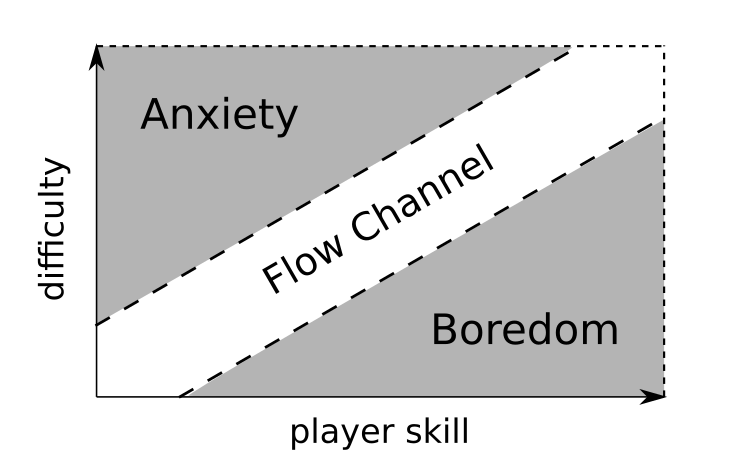
\includegraphics[width=26em]{figures/fig-flow-channel.png}
    \end{center}
    \legend{Source: Diagram assembled by the authors based on the concepts defined by \cite{BOOK_Flow}.}
    \label{fig:flow-channel}
\end{figure}

The balance between challenge and skill strongly contributes to the optimal experience of a player, and is referred to as a defining factor on the quality of a game \cite{ARTICLE_FearOfFailure}. We argue that we can balance the level of challenge through AGT. By acquiring information on the profile and preferences of a player, we can either ramp up the difficulty or encourage the learning process. Therefore, we understand that the usage of AGT can directly contribute to a positive experience.

\subsection{Learning Curve}
\label{sec:learning-curve}

Another interesting concept in games is the \emph{learning curve} \cite{article_learningcurve}. The learning curve depicts how easy it is to become used to the game's mechanics and systems. Game Developers often consider the learning curve as a key reference when performing level design. The first few levels of a game should enable the player to learn each mechanic in an isolated and controlled environment, whereas the last levels of a game should be designed considering that the player has knowledge about all the mechanics proposed by the game designer, and thus should present challenges that require mastery of each mechanic to surpass. Figure \ref{fig:difficulty-curves} depicts multiple possibilities for difficulty curves as a function of player progress in a game.

\begin{figure}
    \caption{Examples of the distribution of difficulty in games as a function of player progress.}
    \begin{center}
        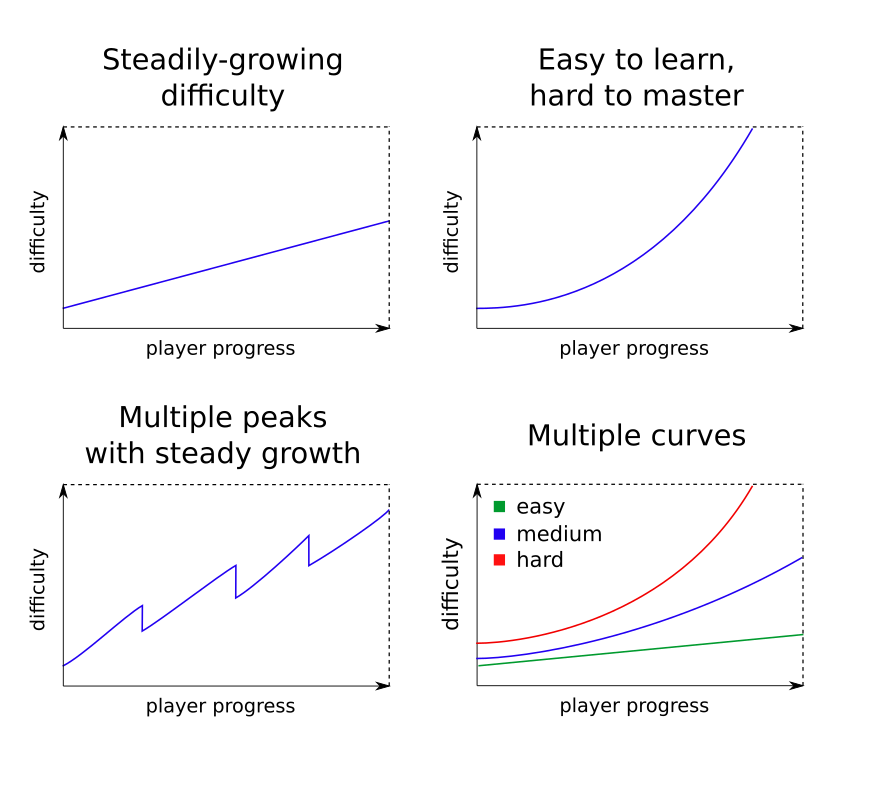
\includegraphics[width=26em]{figures/fig-difficulty-curves.png}
    \end{center}
    \legend{Source: Diagram assembled by the authors.}
    \label{fig:difficulty-curves}
\end{figure}

Perhaps the most notable example in teaching game mechanics through a concise learning curve is seen the famous game \emph{Super Mario Bros} \footnote{Super Mario Bros (Nintendo, 1985). Video Game. Nintendo Entertainment System.} in World 1-1, as addressed in \cite{video_extracreditsmario11}. In the first thirty seconds of gameplay, the player is able to learn that they must progress going to the right, that enemies must be avoided or eliminated by jumping in their heads and that special blocks hide valuable rewards such as additional lives. All the mechanics are taught without a single line of text or on-screen dialog box. Instead, the game teaches them by simply using the player's curiosity with an ingenious placement of game entities.

Some genres of games with consolidated and well-known mechanics share multiple similarities. The mechanics in such genres are proven to be one of the core constituents in their type of gameplay, and are expected by any non-novice player. One example would be the FPS (First Person Shooter) mechanics of \emph{Call of Duty: Modern Warfare}\footnote{Call of Duty: Modern Warfare (Infinity Ward, 2007). Computer Game. Microsoft Windows.}. The running, sprinting, strafing, vaulting, proning and iron-sighting mechanics were so exceptionally well done that they still remain in the most recent title of the series, \emph{Call of Duty: Black Ops 4}\footnote{Call of Duty: Black Ops 4 (Treyarch, 2018). Computer Game. Microsoft Windows.}. Other entries in the FPS genre such as \emph{Battlefield}\footnote{Battlefield 5 (DICE, 2018). Computer Game. Microsoft Windows.} also employ the same set of mechanics, which has since then become almost a requirement for the non-tactical Arcade Shooter style.

Arguably, games with the mechanics of a consolidated genre have a faster initial learning curve to any player that has played a similar game before. These games take advantage of that, and throw the player straight into the action. Within the first few minutes of playing a \emph{Call of Duty} game, the player will have faced and beaten an impressive amount of enemies. They will also confirm their proficiency by choosing exactly the difficulty level that appeals to their skill. Therefore, the veteran player of such a genre knows what to expect of the game and its standard difficulty level. They tailor their game experience to the optimal experience in the act of leisure.

We argue that Adaptive Game Technologies can also have an impact on the learning curve issue. Understanding the profile of a player before gameplay takes place can be a key factor on the decision to ramp up the initial challenge of a game, and remove or alter initial sections which only serve the purpose of teaching basic mechanics.

Thus, the learning curve should not be static, but customized to the needs of each player. If the player has already mastered the base concepts of a game, they should be encouraged to using their knowledge to the fullest. Tailoring the learning experience to each player could balance the challenges faced by the player to a more appropriate, which could possibly increase the sense of enjoyment and immersion as seen in \autoref{sec:challenge-flow}.

% ================================================================================
% ================================================================================
% ADAPTIVITY IN RESEARCH
% ================================================================================
% ================================================================================

\section{Adaptive Systems In Research}

Mechanisms for DDA should describe what elements of the game are going to be monitored, and what variables should be adjusted accordingly. Therefore, the functionality of a DDA system can be summarized as a relation between observation and adjustment. Since video games are so diverse in design and functionality, the mapping between observation parameters and adjustment variables has yet not been efficiently described as an universal and generic approach \cite{PHD_DynamicDifficultyAdjustment}. Rather, the game developer should decide what variables should be observed and adjusted in a per-game basis.

In contrast to the implementations of DDA portrayed in commercial games, prior academic work encompassed a multitude of probabilistic models and data-driven approaches that could prove to be interesting if applied to a commercial solution. In the scope of this work, we use the literary review in \cite{article_ddareview} as a reference to categorize a subset of DDA algorithm variants implemented in previous academic work, as well as to select and perform an analysis on a single relevant representation for each of the proposed solutions.

% =======================================================
% PLAYER MODELING
% =======================================================

\subsection{Player Modeling and Profiling}

The concept of adaptivity in games relates to how a game is able to adapt its content based on the \emph{profile} and \emph{preferences} of a player, which constitute \emph{player models} obtained from a multitude of \emph{Player Modeling} techniques. Player Modeling allows the creation, collection and processing of \emph{player models}, real-time collected data sets that can be classified into reality-based player types \cite{ARTICLE_DynamicPlayerModelling}. Knowledge about player types allows dynamic adjustment in the sense of content customization, where a game designer might dynamically assign what should be presented to each type of player.

In a DDA system, \emph{Player Models} refer to collections of data gathered to be used as a metric for adjustment policies \cite{PHD_DynamicDifficultyAdjustment}. Player Model data might be gathered during a play session as a trace of the player's actions and events in a game, or as static data collected from surveys or through the use of a gaming platform such as \emph{Steam}.

One possible implementation of a \emph{Player Model} consists of defining a collection of numerical attributes that describe the playing style of an individual player, as seen in \cite{BOOK_PlayerModeling}. Each attribute defines an aspect of the player's behavior, which is generally associated with their strategy or mechanical skill. A typical example of Player Model in a Shooter game can be seen in Listing \ref{lst:PlayerModellingExample}.

\begin{lstlisting}[caption={Example of a Player Model for a shooter game.},label={lst:PlayerModellingExample}]
class PlayerModel {
  public:
    enum Attribute {
      bCanStrafe,
      bCanFlick,
      bDoesStationaryShooting,
      fPrecision,
      fEncounterDuration,
      fKillsPerRound,
      fDamagePerRound,
      fDistancePerRound
    }
    void Initialize();
    void UpdateAttribute(Attribute att, float newValue);
    float GetAttribute(Attribute att);
    private:
      vector<float> attributeValues;
};
\end{lstlisting}

The values for each attribute are unknown to the game preceding a session. Therefore, it is necessary to sample and adjust the values during gameplay. Each time a sample is collected, the Player Model should reflect a player's behavior with increasing precision. In the implementation proposed by \citet{BOOK_PlayerModeling}, the attribute update function uses the \emph{Least Mean Squares} (LMS) training rule, commonly used in machine learning:

\begin{lstlisting}[caption={Implementation of attribute update using least mean squares.},label={lst:AttributeUpdate}]
float UpdateAttribute(Attribute att, float value) {
    float currvalue = attributeValues[att]; N
    float delta = value - currvalue;
    float weightedDelta = LEARNING_RATE * delta;
    attributeValues[att] += weightedDelta;
}
\end{lstlisting}

Attributes in this implementation consist of values between 0 and 1, indicating the probability of a player performing an action. In Listing \ref{lst:PlayerModellingExample}, this can be seen in the definitions of Boolean attributes (prefix 'b'). However, it is also possible to use the same approach to approximate statistical values, such as the damage a player inflicts per round. The value for each attribute represents the game's current best guess. Each sample collected contributes to the estimate weighted by LEARNING\_RATE. Therefore, for lower LEARNING\_RATE values more samples are required to sufficiently approximate an attribute. In most cases, values between 0.1 and 0.3 are used \cite{BOOK_PlayerModeling}.

Another perspective brought to the concept of player models is seen in \cite{ARTICLE_DynamicPlayerModelling}, where the authors describe a Player Modeling framework that takes \emph{concept drift} into consideration, which is the possibility of players adapting or changing behaviors and play styles according to their evolution or progress in a game. The framework relies on two sources of player-related data: information of player preferences inputted by a player prior to application use and tracking player performance in-game. Figure \ref{fig:dynamic-player-model} exemplifies the dynamic player model framework.

The discussion in \cite{ARTICLE_DynamicPlayerModelling} emphasizes the necessity of remodeling player types after measuring the effectiveness of adaptation. This means that a DDA system should be able to gather some type of player feedback regarding the effectiveness of the dynamic adjustments that were performed during play, and recreate the player profile based on this feedback. Some methods for gathering such feedback include inferring the player's affective state, such as with physiological sensors or from a camera or an analysis of statistical data retrieved from in-game attributes, such as player performance or their action history.

\begin{figure}[!ht]
    \caption{A representation of the dynamic player modeling framework discussed in \cite{ARTICLE_DynamicPlayerModelling}.}
    \begin{center}
        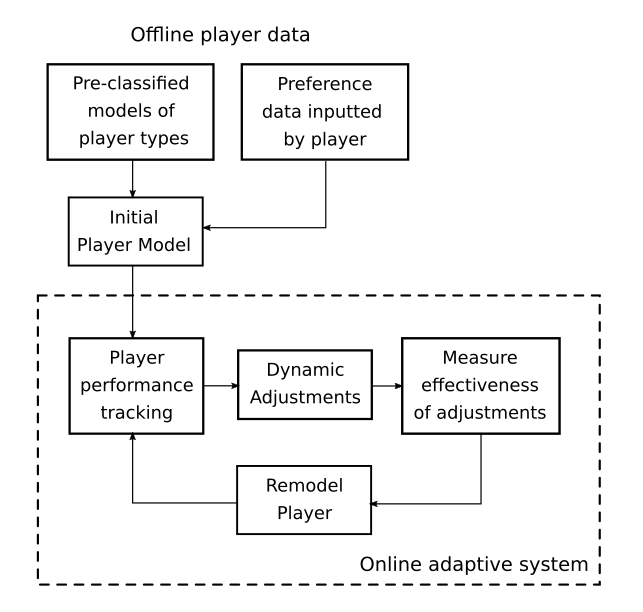
\includegraphics[width=26em]{figures/fig-dynamic-player-model.png}
    \end{center}
    \legend{Source: Diagram assembled by the authors based on visual representations in \cite{ARTICLE_DynamicPlayerModelling}.}
    \label{fig:dynamic-player-model}
\end{figure}

% =======================================================
% PROBABILISTIC DDA
% =======================================================

\subsection{Probabilistic DDA Systems}
\label{sec:statistical-adjustments}

One of the first and most relevant implementations of the probabilistic model approach for DDA systems is the Hamlet system seen in \cite{article_casefordynamicdifficulty}. Hamlet is a probability-based predictive system that is able to perform reactive and proactive adjustments to the distribution of items throughout levels of customized Half-Life \footnote{Half-Life (Valve Software, 1998). Computer Game. Microsoft Windows.} map \cite{article_casefordynamicdifficulty}. The system works by defining a finite set of possible game world states, and performing adjustments with the objective of avoiding game state "loops", where a player would perform the same set of actions repeatedly.

First, Hamlet establishes the probabilistic distribution of damage done to the player using a series of measurements taken over time. By doing this for each of the enemy classes, the probability of the player dying during an encounter can be estimated. Then, if the probability of death for an encounter is above 40\%, the system intervenes by distributing \emph{healing items}\footnote{Healing items in games are consumable resources that restore a percentage of the maximum health points of a player. An example for this are the health stations in the Half-Life franchise, where the player heals up to 80\% of their maximum health points upon interaction, but the resource is permanently depleted after use.} throughout the level before an encounter takes place. This is an example of \emph{proactive adjustment}, which occurs before an in-game event takes place. The author of the article argues that the effectiveness of proactive adjustments is harder to measure than \emph{reactive} adjustments, and thus this type of adjustment should be performed based on predefined constraints determined by the game designer.

Hamlet is also able to perform \emph{reactive} adjustments that occur during combat encounters, such as adjusting the maximum hit points for an enemy class or modifying the accuracy of enemy shots. The objective of any adjustment is to decrease the amount of player deaths for each level independently of player skill, and to achieve a mean health percentage of 60 with a standard deviation of 15 points at any given point.

Results of the experiment using the Hamlet system showed that most players were unable to recognize when the system was performing adjustments, or characteristics of the game were modified when adjustments were performed. Some players suggested that the system performed adjustments that were not there, and several players suggested that the system did not perform any adjustments based on their skill level. During the post evaluation interviews, there was a slight correlation between the adjustment policies and player enjoyment when considering players with expert skill level, although players with novice skill level did not report any perceivable change.

The study concluded that adjustment algorithms can include the performance of a player while retaining the player's sense of agency and control. When performed with accordance to the game's core design, adjustments can be nearly imperceptible, and slightly increase the sense of enjoyment of a player without diverging from the proposed experience.

Therefore, the Hamlet system proposed by \citet{article_casefordynamicdifficulty} addresses the possibility of predicting gameplay outcomes given a game world state, and performing \emph{reactive} or \emph{proactive} adjustments for a more immediate resolution when compared to other solutions. We argue that while this might be an interesting approach for a supportive or secondary DDA system, this type of solution might be hard to tailor from a game designer's perspective since it is impossible to predict results functionally.

% =======================================================
% AFFECT-BASED DDA
% =======================================================

\subsection{Affect-based DDA Systems}

Most implementations of DDA systems use as adjustment policies metrics that would represent player performance. However, the affective state experienced by players could also play a key role in the gaming experience, and thus could be a useful metric for adjustment policies in DDA systems. This is the theme of the work presented in \cite{article_affectivedda}, where physiological signals were tracked to infer the anxiety level of players, and then used as a metric to perform dynamic adjustments.

The work of \citet{article_affectivedda} cites previous research indicating that electrodermal and cardiovascular activities had a relation to anxiety levels. An increase in skin conductance may be caused by anxiety. A decrease of parasympathetic activity and increase in sympathetic activity in the heart also may suggest anxiety \cite{article_affectivedda}.

Blood pulse volume measured at fingers were also shown to be subject to stress manipulation, and presents a correlation with self-reported anxiety \cite{article_affectivedda}. Measures of EMG (Electromyography) activity of specific muscles (such as Corrugator Supercilii) were also shown to be strong indicators of anxiety.

Therefore, the work presented in \cite{article_affectivedda} used features of cardiovascular activity, such as interbeat interval, relative pulse volume, pulse transit time and heart sound; electrodermal activity (tonic and phasic response to skin conductance) and EMG activity (from Corrugator Supercilii, Zygomaticus and upper Trapezius muscles) as input measures to a Regression Tree (RT) technique which classifies the physiological signals into affective states that categorize anxiety levels.

A Pong-based game was implemented for the study, with two variations in difficulty adjustment algorithm: one where the difficulty would be adapted based on player performance (a relationship between points scored against or in favor of the player), and another where the anxiety level of the player is used as input to alter difficulty.

Three difficulty levels were implemented in total, which would be assigned depending on performance or anxiety levels: if the player's performance is classified as "Excellent", the player would progress into the next difficulty level. If the performance is classified as "Poor", the difficulty level would be decreased. The affect-based variant utilizes an analogue solution, where the difficulty is increased if the anxiety level is classified as "Low", and the difficulty is decreased if the anxiety level is classified as "High". Figure \ref{fig:affective-adaptation} displays state-flow diagrams representing the difficulty levels and their transition conditions.

\begin{figure}[!h]
    \caption{A state-flow diagram representation of the performance-based and anxiety-based adaptation variants in \cite{article_affectivedda}.}
    \begin{center}
        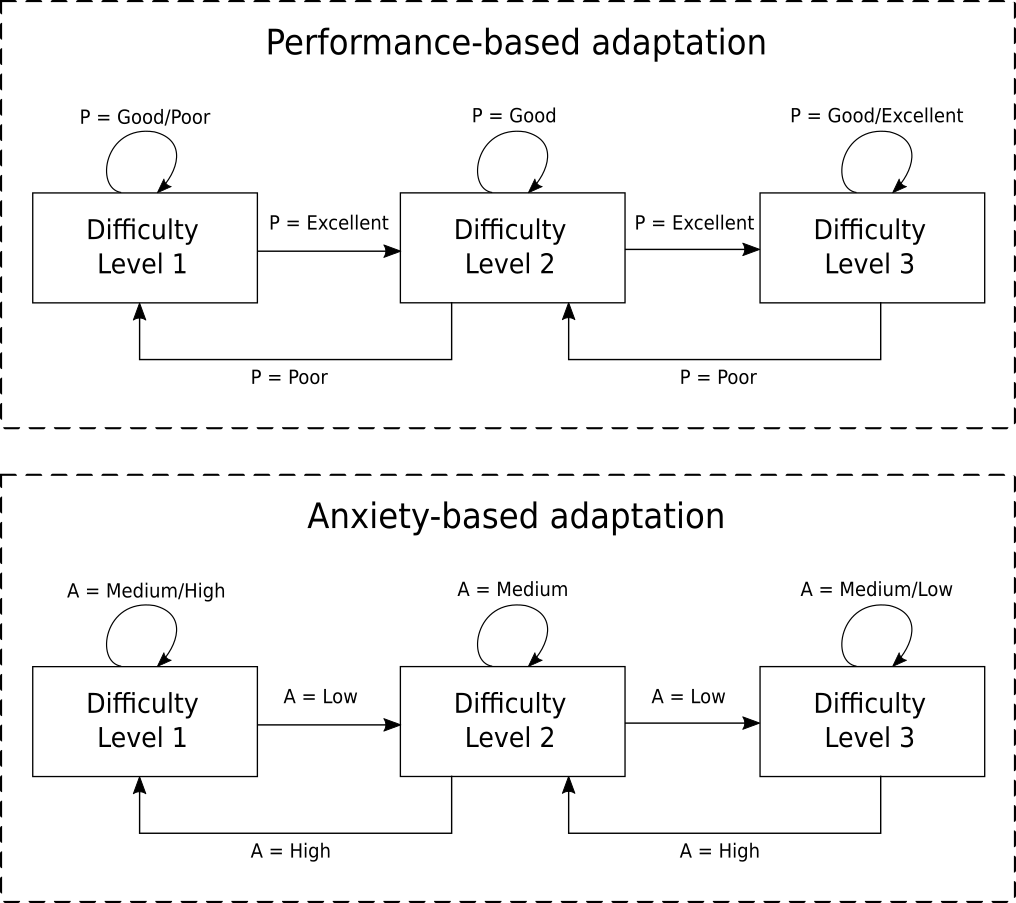
\includegraphics[width=26em]{figures/fig-affective-adaptation.png}
    \end{center}
    \legend{Source: Diagram assembled by the authors based on visual representations in \cite{article_affectivedda}.}
    \label{fig:affective-adaptation}
\end{figure}

The results of the experiment showed that the performance of most players improved during the affect-based DDA session in relation to the performance-based DDA session. Players also perceived the affect-based DDA version to be more challenging than performance-based DDA, and reported that the affective version was more satisfying.

We argue that, while the results of the experiment portrayed in \cite{article_affectivedda} showed mostly positive results in comparison to performance-tracking DDA, employing this type of solution in a commercial video game is not feasible, as current hardware is unable to track physiological signals in a significant way. 

Furthermore, the game implementation used for the experiment is a simplistic game with limited audiovisual feedback. Therefore, a similar experiment could be performed in a modern game with high audiovisual fidelity to evaluate results, as modern games are often able to evoke a multitude affective reactions by immersing the player in a \emph{cutscene}\footnote{A \emph{cutscene} is a special in-game event where the player is unable to input control into the game, and audiovisual feedback is a result of an automatic, predefined sequence of events determined by the game developers. Cutscenes can be seen as parts of a game that are similar to a movie, where the game is not interactive and instead focuses on telling a part of the story.} or a series of chaotic events.

% =======================================================
% LEARNING-BASED DDA
% =======================================================

\subsection{Reinforcement Learning in DDA Systems}

Another approach to adaptive difficulty involves the adaptation of AI (Artificial Intelligence) agent behaviors through reinforcement learning, as exemplified in \cite{article_adaptivebehaviorai}. Their implementation defines AI agents in a simple car simulation race game, where each player has the objective of passing through the maximum number of \emph{waypoints}\footnote{A \emph{waypoint} is a special position in a game world where an in-game event is toggled when the player is within interaction range. Waypoints are commonly used in games when the player has to take a specific path to a goal, with the game assigning several intermediary positions the player has to pass through to validate that the correct path was taken. In the context used for the implementation presented in \cite{article_adaptivebehaviorai}, waypoints are simply game world positions the cars must reach to score points. Each time one of these positions is occupied by a car, the waypoint is destroyed and a new random position is assigned elsewhere in the game world as the next waypoint.} in a given amount of time. Multiple waypoints are displayed on the screen at any given time, and a waypoint disappears when any of the players is within interaction range.

The AI agents implemented in \cite{article_adaptivebehaviorai} define two layers of behavioral AI components. The first layer contains components associated with driving functionality, with the objective of improving driving performance of the controller. The second layer is associated with tactical behavior components that seek to outplay the opponent in the game.

Driving behavior components ignore the existence of the opponent, leading to inferior performance in the game. Tactical behavior components help the AI controller decide which waypoint to head to, or if the controller should not head to a waypoint at all. In more general perspective, the Driving Behavior components can be seen as the mechanical input of AI agents in the game, whereas the Tactical Behavior components could be considered the high-level decision making components of the AI.

To evaluate the performance of adaptive AI agent controllers, two evolutionary computation algorithms are implemented: the adaptive uni-chromosome controller (AUC) and the adaptive duo-chromosome controller (ADC). The advantage of using such algorithms is that the training and adaptation process occurs in real time during the course of a game session.

Each chromosome in said algorithms stores seven real numbers representing the probability of activating a behavioral component whenever a waypoint is passed. Two metrics are used as an input for the adaptation algorithm: first, a minimization of the winning percentage difference (|W - L|, where W represents the wins and L represents the losses) and second, a minimization of the mean score difference (|s1-s2| where s1 and s2 represent the scores of player 1 and player 2).

To evaluate the efficiency of the proposed algorithms, the authors first compared the strongest AI agent that the adaptive system would possibly generate (defined by enabling all behavioral components simultaneously and permanently) against five static AI controllers based on various traits that would simulate various styles of play, such as heuristic controllers, reverse-enabled controllers, predictive fast controllers, and neural network controllers.

Sets of \emph{n = 5000} games were played for each opponent in each step of the experiment. Through the first step of the experiment, the authors validated that a fully-enabled adaptive AI controller (having all the behavioral components activated at all times) was a competent opponent with positive median score differences against all static AI controllers.

In the second step, the behaviors were activated randomly whenever a waypoint was crossed to demonstrate that an effective adaptation algorithm is necessary for different types of opponents. Results showed that the random behavior selection algorithm had negative median score differences against all five static controllers.

In the third step, the authors evaluate the use of the AUC algorithm. The expected behavior set encoded by a chromosome as a result of the algorithm should represent a "winning" strategy. Effects of varying \emph{Learning Rate} and \emph{Mutation Rate} were documented for the experiment, showing that the general trend of increasing learning rate is a gentle increase in the mean score difference, since a large learning rate quickly saturates chromosome values to either 0 or 1. Higher mutation rates tend to produce larger differences in mean score and winning percentage by producing large fluctuations in chromosome values. In general, high mutation rates led to poorer results, and the optimal value of 0.1 was stated for the AUC algorithm variant.

In the final step of the experiment, the use of the ADC algorithm is evaluated, with the same idea of varying the Learning and Mutation Rates. For the ADC algorithm, no trends were perceived in association with varying Learning rates. This would likely have been caused by the reduction of the frequency of update opportunities for each chromosome. In the ADC algorithm, only one of two chromosomes is updated each time a waypoint is passed. This means that on average each chromosome is updated half as frequently as chromosomes in the AUC variant. As for the Mutation rate, the results of the ADC controller improved greatly as mutation was introduced, possibly because the mutation operation offered more opportunities for the chromosome values to adapt.

As a conclusion to the experiment, the authors expressed that while the AUC algorithm had lower memory footprint, the ADC algorithm was able to better minimize the number of drawn games, which would possibly reduce player frustration. It was also noted that both the AUC and ADC algorithms were able to generate specific patterns of behavioral component distribution for each of the static controller stereotypes, meaning that the Reinforcement Learning technique would be able to adapt to different styles of play. The general intent of both algorithms was not to maximize the number of wins, but to maintain a fair and close challenge to the opponent by minimizing the score difference as well as the difference between number of wins and losses.

The work presented in \cite{article_adaptivebehaviorai} introduces the novelty approach of online learning without predefined data sets to the scenario of DDA solutions. It could be argued that the adjustment policies are also part of the reinforcement learning approach, since the decision of a behavioral component being activated or not relies on the algorithm being applied. This is an especially interesting solution since it lessens the responsibility of a game designer tailoring the boundaries of the adjustment system in advance of play. However, we argue that this experiment has yet to be applied in the context of real players using an implementation that would better replicate a commercial video game product.

% ================================================================================
% ================================================================================
% ADAPTIVITY IN COMMERCIAL GAMES
% ================================================================================
% ================================================================================

\section{Adaptive Systems In Commercial Games}

Several commercial games have attempted to create Dynamic Difficulty systems which embrace varying degrees of player skill, such as \emph{Mario Kart} \sepfootnote{fn:mario-kart}, \emph{Half-Life 2} \sepfootnote{fn:half-life-2}, \emph{Resident Evil 4} \sepfootnote{fn:resident-evil-4} and \emph{God Hand} \sepfootnote{fn:god-hand}. In this section, we look at examples of Adaptive Systems in some of the most popular games developed by the video game industry in the last decades. We categorize the solutions based on which game systems they affect, and discuss some of the caveats of each system.

% =======================================================
% RUBBER BANDING ADAPTIVITY
% =======================================================

\subsection{Rubber-banding in Mario Kart}
\label{sec:rubber-banding-mario-kart}

Perhaps the most popular approach to Adaptive Difficulty is found in games which present \emph{rubber banding}. This technique is most commonly seen in racing games that have artificial intelligence agents as opponents to the player. If the player performs exceptionally well in a race and is far ahead of every AI opponent, the opponents will receive a significant speed boost that often surpasses the standard speed limits of the game. In case the player performs poorly, the AI is slowed down below their base speed so that the player is able to catch up. The term \emph{rubber banding} derives from the analogy that the players and their opponents are held together by a rubber band, so that they are never too far apart from their opponents.

Rubber banding is employed to cause the impression that the outcome of the race is never clearly defined, enabling the perception that mistakes by the competitor that is ahead can greatly affect their chances of winning. The existence of the rubber banding system, along with the perception caused by it, results in the increase of tension and focus by the player. Rubber banding is not limited to the Racing games genre, and it does necessarily happen only between players and AI. However, it does imply that the game has some sort of competition system, even if the game is a single-player \footnote{A single player game is a video game where the input processed by the game is received from only one human user (player) during the course of a game session. All entities the player interacts within the game world are non-player entities.} or cooperative \footnote{Cooperative games are games in which the input is received from multiple human users (players), with each player controlling a different in-game entity. The players share a common objective, and must cooperate by combining their available commands and actions to achieve the winning condition.} experience.

Mario Kart applies rubber banding through two different methods, affecting both players and computer-controlled opponents \cite{website_rubberbandingmariokart}. The first type of rubber banding compares the performance of players to AI opponents: if a player is too far behind the computer-controlled opponents, the AI slows down by lowering their maximum speed. If a player is too far ahead, the AI receives a significant speed boost to their base speed. While being a simplistic solution common to many games in the racing genre, it attenuates the skill discrepancy between players and AI. 

The second solution in Mario Kart is presented through the power-up system, and targets the issue of skill discrepancy between players. Throughout the race, players are provided with multiple randomly-generated power-ups, which can be used to speed-up, attack or defend against opponents. Speed-up pickups are favored to players who are far behind others, whereas attack and defense power-ups are favored to players who are closer to attaining the first position. Players in the first position are generally provided the worse pickups. This provides better opportunities for players who are lower-skilled, as the access to speed power-ups is limited to the competitors who are far behind, and effectively serves as a catching-up mechanic.

While this solution is an interesting and creative effort that makes matches between players of varying skill levels more competitive, players that become aware of this system might avoid the first position to retain the best power-ups until the last moments of a race. This situation elicits the problem of meta-gaming in adaptive systems: when the adaptive systems are well-known by the users, exploits become a part of player strategy.

% =======================================================
% ENEMY BEHAVIOR & ITEM DISTRIBUTION ADAPTIVITY
% =======================================================

\subsection{Dynamic Items, Behaviors and Levels in Resident Evil 4}

\sepfootnotecontent{fn:re4-gameplay-description}{Footnote: What is Resident Evil 4 in terms of gameplay}

\sepfootnotecontent{fn:skill-ceiling}{Foonote: What is Skill Ceiling}

%   - In RE4 Level layouts, AI behavior and item distribution are affected by player performance 
Another interesting approach to adaptivity is seen in \emph{Resident Evil 4}\sepfootnote{fn:re4-gameplay-description}, where item distribution, AI behavior and enemy encounters are affected by different sets of information regarding player context and performance. Each system is affected by a different set of contextual metrics, and may enable or disable certain gameplay aspects independently based on the values presented by such metrics.

\subsubsection{Dynamic Item Distribution}

% ============================
% How the Dynamic Item Distribution System works
% ============================
%   - Dynamic Item Distribution Affects RNG systems by modifying loot tables based on player needs at a given context
%   - When player has low health, item distribution prioritizes health items
%   - If player has surplus ammo & health, prioritizes gold coins
%   - Veteran players control the use of resources 
The \emph{Dynamic Item distribution} System affects RNG (Random Number Generation) systems by modifying the chances of certain items being distributed when a player interacts with containers or defeats an enemy. The list of items which have their spawn chances modified depends on the current status and context of the player such as their health and the items in their inventory.

For instance, if the player has a low amount of health and no health recovery items in their inventory, the Dynamic Item Distribution system modifies the chances of health recovery items being distributed. If the player has a stabilized amount of health but lacks a specific ammunition type, the game prioritizes the distribution of such ammunition type for the player. If the player is not in a dangerous situation and has surplus ammunition, the game prioritizes gold coins, which can be used to purchase powerful weapons and weapon upgrades. 

% Benefits of Dynamic Item Distribution
% ============================

% - One of the most prevalent types of systems due to:
%   - Easy to implement, as it just modifies chances
%   - Easy to understand by game designers
%   - Ease of abstraction
%    - On a first playthrough, hard to perceive RNG
%    - On RNG systems, hard to tell what factors can influence the loot table
% - Can be integrated into the iterative game design process
% - Balancing values can be replicated throughout game sections 
In the landscape of commercial games, Dynamic Item Distribution Systems are one of the most prevalent adaptive systems types, due to:
\begin{itemize} 
    \item{Their ease of implementation, which involves monitoring of contextual values for player status and performance and simple modification of statistical values;}
    \item{Their straightforward process of adjustment, in which the values can be easily understood and tailored by game designers between playtests;}
    \item{The possibility to integrate them in the iterative nature of the game development process, where values can easily be adjusted between multiple play sessions;}
    \item{The fact that the balancement of item distribution can be replicated througout multiple sections of a game;}
    \item{The fact that they are abstract in nature, meaning that players have difficulty recognizing their existence or the complete extent of the modifications they perform.}
    \item{Their relation with RNG item distribution chance tables, where the factors that influence the chances for each element are ambiguous even for veteran players.}
\end{itemize}

% Examples of Dynamic Item Distribution in Other Games
% ============================

% Examples of other successful games that use dynamic item distribution
%   - Half Life 2
%   - Left 4 Dead
%   - Diablo
Examples of other successful games that also use Dynamic Item Distribution Systems include \emph{Half-Life 2}, where resources are spawned in containers such as destructible boxes based on player health and ammunition; \emph{Left 4 Dead}, where the spawn points of weapons, ammunition and health kits are toggled in fixed spots based on how well the team is performing throughout a level; and \emph{Diablo}, where the rarity of items dropped by defeated enemies depends on the level, modifiers and rarity of the enemy.

% - Can help beginner players 
% - Highly skilled players are rewarded for their performance
In the specific case of Resident Evil 4, Dynamic Item Distribution may benefit beginner players by providing a steady supply of health and ammunition resources during sections of the game with intense combat encounters. The system always prioritizes the most important necessity for the player at a given moment, and as players are able to defeat enemies during a combat encounter, they are be supplied with ammunition and recovery items to be able to continue through a battle. For higher skilled players which are able to maintain a steady level of resources at their disposal, the game rewards performance with gold coins, which enables weapon upgrades that increase the efficiency at which the player is able to dispose of enemies. 

% Problems with Dynamic Item Distribution
% ============================

% - Beginner players could benefit from item hoarding
% - Important resources may not be distributed at critical sections of the game

% In harder sections of the game, beginner players generally need a high amount of resources due to the large amount of enemies being spawned and the lack of knowledge on how to deal with enemies
% As the player defeats enemies, loses health and spends ammunition, resources are constantly depleted from their inventory
Some of the problems involving the implementation of Dynamic Item Distribution in Resident Evil 4 can be analyzed through the perspective of beginner players when facing challenging sections of the game. In such sections, beginner players generally need to spend a higher amount of resources due to the large amount of enemies and their lack of knowledge on how to dispose of multiple enemies. As the player progresses through the combat encounter, they will likely lose significant amounts of health and ammunition. Therefore, resources will be constantly depleted from the player inventory, which is an expected result from the perspective of the Dynamic Distribution System. 

% At an initial point of a combat encounter, enemies would most likely drop less necessary resources such as gold coins
% Player may start to run out of resources at a critical point in the encounter, such when as when facing tougher enemies that are harder to dispose of
However, the main problem with resource distribution becomes evident when considering the flow of events in challenging combat encounters. Generally, at an initial point of the encounter the easiest enemies are spawned, and will most likely drop less necessary resources such as gold coins when defeated. After multiple waves of enemies the player may start to run out of resources, and at the same time progresses closer to the critical points in the encounter, such as facing special enemies that are harder to dispose of.

Since resource distribution is limited to the events of destroying containers and defeating enemies, beginner players that are unaware of the resource distribution system might destroy all containers at the beginning of an encounter, which causes the only resource distribution source to be the defeated enemies. At that point, tougher enemies which cause the player to generally lose more health and spend more ammunition might drain the player of all their resources before they are defeated.

% In conclusion, beginner players could benefit from the possibility of item hoarding for such encounters, which is harder to achieve due to the way dynamic item distribution is implemented
In such situations, a beginner player would benefit from the ability to perform \emph{item hoarding}, where the player accumulates resources over easier sections of a game to be spent on the more challenging levels. Because of the way item distribution is implemented in Resident Evil 4, item hoarding becomes harder to perform, since as the player accumulates health or ammunition resources the game will prioritize distributing low necessity items such as gold coins.

% - Players may choose to not loot resource items purposefully
%   - Force the system to generate resource items only at critical sections of the game
%       - Maximize inventory space for weapons
%       - Maximize the money gained for upgrades
Additionally, a player that is aware of an adaptive distribution system might exploit the game by choosing to not loot items purposefully. By maintaining their resources at a controlled level, veteran players can prioritize the use of their inventories for important weapons and items, and force the system to distribute important resources at critical points in the game such as before an encounter with a large group of enemies. However, it can be argued that this characteristic can also be a benefit to highly skilled players, where good management of resources throughout the game can lead to rewards in terms of combat performance, as the player will possess better weapons and upgrades at their disposal.

\subsubsection{Dynamic AI Behaviors}

% ============================
% How the Dynamic AI Behavior System works
% ============================

%    - Affects the actions performed by AI agents
%    - Based on player performance and habits
The \emph{Dynamic AI Behaviors} system affects the actions performed by AI-controlled entities based on player performance and habits. In Resident Evil 4, players are able to increase their damage output and cause enemies to become staggered and unable to attack by shooting at their heads. When staggered, the player can also perform a \emph{kick attack}, which causes enemies to fall into the ground for a significant amount of time. 

%    - If player constantly headshots, enemies start to dodge, defend head & equip armor
If a player is constantly able to defeat enemies easily by shooting their heads or without spending significant resources such as ammunition and health recovery items, enemies will start to perform new actions such as attempting to dodge or even using their hands to block bullets. Additionally, enemies in later stages of the game will also equip protective apparel such as helmets and shields depending on player accuracy, which hinders the ability of the player to deal damage and cause staggers.

% - Experienced player can still be effective even with AI changes
Although the new actions and equipment presented by enemies can become an obstacle for effectiveness, they are not overwhelmingly difficult to handle. An experienced player can still be effective and shoot enemy heads with precision if they are able to predict enemy movement, react to character animations and use the proper weapons for each equipment.

% TODO Examples of Dynamic AI Behaviors In Other Games
% ============================



% Benefits of Dynamic AI Behaviors
% ============================

% - Instead of making game super difficult, focuses on increasing skill ceiling
Therefore, instead of simply increasing the difficulty to an overwhelmingly high level of challenge, the implementation of Dynamic AI Behavior System in Resident Evil 4 causes the game to increase its skill ceiling\sepfootnote{fn:skill-ceiling} in an interesting way, enabling interesting situations in enemy encounters that can provide variety and challenge for experienced and highly skilled players.

% - The new actions performed by enemies are in-world elements that contribute to the believability of enemy behaviors, giving the sense that they become more intelligent to deal with the player over time and improves immersion
Additionally, the new actions performed by enemies after Dynamic Behavior adjustments are in-world elements that contribute to the believability of enemy behaviors, since they aesthetically portray the intent that enemies are trying to protect vulnerable body parts from player firearms. Therefore, instead of the player perceiving the new actions as part of a system, they are given the information that enemies are progressively becoming more intelligent to be able to deal with the player, which improves immersion.

% - The armor pieces that are equipped by enemies at later sections of the game presents harmony with the thematic difference in comparison to earlier sections
% - In earlier sections, enemies are farmers, which are less likely to wield any type of armor
% - In the middle sections, player is in a castle and enemies start wearing shields and helmets, but not full body armors
% - In the later sections, enemies are rebel soldiers which use proper protective equipment against heavy firearms
In regards to the adaptivity of armor pieces wielded by enemies, the equipment used in later sections of the game presents harmony with the thematic aspects of the environment in comparison to preceding sections. In the early sections of Resident Evil 4, the player traverses through small villages in a rural environment where most enemies are farmers, and thus less likely to wield any type of armor. The second segment of the game is located within a castle, where enemies are more likely to wield specific armor pieces such as shields and helmets, which protects them from attacks targeted at their body and head, respectively. In the final segments of the game, the player faces enemies that represent rebel soldiers, which wield protection that is effective against heavy firearms. Therefore, the adaptivity in enemy equipment can easily be abstracted by the player given the thematic context of each game segment.

% Problems with Dynamic AI Behaviors
% ============================

% - Use of Game Rank
% - Metrics of Game Rank are displayed after level is finished
% - The exposure of metrics can expose the adaptivity to players
% TODO RE4_JP_StrategyGuide: Pages 23-26
To implement the Dynamic AI Behavior System, Resident Evil 4 uses a skill rating system called \emph{Game Rank}, which is increased or decreased according to aim precision and level completion time \cite{RE4_JP_StrategyGuide}. The metrics that constitute Game Rank are exposed to the player after the completion of each level, and aggregated to a final rating score. The fact that the existence of such metrics is explicit to players can be a detrimental factor when combined with the gameplay aspect of new actions performed by enemies when players achieve a highly positive performance.

% - The intent of enemy animations is easily perceivable by players when trying to aim at their heads
% - The combination of these factors caused the system to be quickly perceived by players
% - Veterans & Speedrunners exploit game rank by missing on purpose
% - Game then constrains enemy behaviors to predictable movement
While protective enemy animations can be considered in-world elements that contribute to player immersion, it can be argued that since they purposefully communicate their intent to players, there is an increase in the chance of the player being able to recognize and correlate the existence of new enemy actions with the metrics exposed after the completion of levels. Veteran players and \emph{speedrunners} often exploit Game Rank by missing shots on purpose, artificially lowering their precision value. This causes the game to constrain enemy behavior to predictable movement patterns, where shooting enemy heads is easier than in a standard play through.

% - This is another example of players exploiting adaptivity
This is another example of meta-game strategies in adaptive solutions, where players that are knowledgeable of the adaptive systems attempt to exploit it to constrain the behavioral patterns of AI agents. In comparison to the example discussed about the distribution of power-ups in Mario Kart in section \ref{sec:rubber-banding-mario-kart}, exploitability in Dynamic AI Behavior Systems have a less relevant collateral effect since such systems are commonly restricted to \emph{single-player} games, where the decisions of a player do not affect the outcomes of actions for another player. However, players that have knowledge of Dynamic AI Behaviors might still be able to modify their playing style to manually adjust the challenge level and make certain segments of the game easier, which goes in disagreement with the level of challenge proposed by game designers and causes the player to break their own immersion.

\subsubsection{Dynamic Encounters}

% ============================
% How the Dynamic Encounters System works
% ============================

\sepfootnotecontent{fn:joystick-controllers}{Footnote: What are joystick controllers}

% - Modifies placement of enemies
% - Triggered by repeated deaths at certain sections of the game
% - Enemy spawns are enabled or disabled according to performance
The \emph{Dynamic Encounters} System modifies the placement of enemies in levels, affecting the difficulty of encounters by enabling or disabling the instantiation of certain enemies in game sections where the player engages a combat situation. If the player repeatedly dies in a specific combat encounter certain enemies spawns are disabled, making the encounter much less frustrating. 

% - Long range enemies are the hardest to deal with, since generally require sniper rifles
% - Sniper rifles are slower and harder to aim with, melee enemies can close the distance
In general, long range enemies such as crossbow wielders which are hard to reach or take a longer amount of time and resources to eliminate are the first to be disabled since there is no direct or easy method for the player to avoid them. Additionally, the best weapon type to deal with enemies at a long distance would be the \emph{sniper rifles}, which are bound to long aiming animations and slow crosshair movement. Since the player is unable to perform movement while aiming in Resident Evil 4, enemies wielding melee weapons are able to close their distance to the player during the time where the player attempts to aim at a long range target.

% - Ambush enemies that are spawned outside player FOV
% - If player is doing well, higher chance for them to spawn
% - Make challenge higher instead of easier
% - Hard to react to
The second type of adjustment performed by the Dynamic Encounters System involves the appearance of ambush-type enemies, which only spawn outside of player field-of-view. If the player is performing well and accumulates a significant amount of health resources, ambush-type enemy spawns are enabled to cause the perception that even though the player is skilled enough to deal with enemies in direct combat, there are still traps and surprising situations that might cause the player to be defeated. Contrary to the removal of long range enemies when the player repeatedly dies, ambush-type enemies are designed to drain the player of resources and increase the tension throughout levels. Since these enemies are harder to perceive, they will often be harder to react to and cause the player to perform incorrect actions or input.

% Benefits of Dynamic Encounters
% ============================

% - Dynamic Encounters are one of the best solutions for cases where the player requires some sort of assistance in the form of immediate adaptation, such as when a player is repeatedly failing a level. Changes in the placement or number of enemies can greatly affect the level of challenge of a combat encounter, and the entities that cause the most impact can be directly removed, which significantly helps players to overcome specific sections

% - 

% Problems with Dynamic Encounters
% ============================

% - Modifications in encounters based on the number of deaths in that specific encounter are the easiest to perceive, as when repeatedly playing through a same section the player is able to memorize enemy positions and movement patterns
% - Players might feel frustrated with the fact the the game forcefully lowers the difficulty without their consent, meaning that the game implicitly classifies the player as unable to deal with an encounter

% - Dynamic Encounters are one of the adaptive systems most sensitive to modifications, since small changes in the placement or number of enemies can greatly magnify the increase or decrease of difficulty caused by other game elements which are difficulty factors, such as AI Behaviors, or the damage dealt by an enemy type 
% - Due to being sensitive to modifications, Dynamic Encounters are one of the hardest adaptivity methods to balance, since they require per-encounter play testing and iteration through multiple contexts to appropriately increase or decrease the level of difficulty based on player performance 

% Unused yet
% ============================
% While Resident Evil 4 received mass critical praise for its outstanding game design and successful adaptive approach, it is noteworthy that a community of dedicated \emph{speedrunners} has been able to accurately reverse engineer and exploit its DDA systems \sepfootnote{fn:speedrun-com-re4-guides}. It can be argued that given enough dedication, there is no DDA system which is completely unknown to players. However, since the reverse engineering process requires extensive experimentation on behalf of players, we can assume that the system will remain mostly obfuscated to novice players experiencing their first play through, which is critical to maintain immersion and player engagement.

% =======================================================
% EXPLICIT ADAPTIVITY
% =======================================================

\subsection{Explicit Adaptivity in God Hand}

\sepfootnotecontent{fn:god-hand-gameplay-description}{Footnote: What is God Hand in terms of gameplay}

% How the system works
% ============================

% - In God Hand difficulty is explicit
% - Difficulty meter in UI with 3 difficulty levels
% - Higher difficulty levels introduce new behaviors, faster enemies, more damage received
% - Difficulty decreases when the player is hit
In \emph{God Hand}\sepfootnote{fn:god-hand-gameplay-description}, the developers approached the difficulty issue explicitly by making the player constantly aware of the current challenge level \cite{article_subjectivedifficulty}. A difficulty meter is presented to the players as an User Interface element containing 3 difficulty levels. Whenever the player hits an enemy, the meter slightly increases. When the meter is full, the difficulty level is incremented and enemies become faster, introduce new behaviors and deal more damage. When the player takes damage, the difficulty meter is quickly decreased and will often reduce the current difficulty level.

% - In max difficulty, enemies hit faster than player can dodge
% - When player beats enemy, they are rewarded with points based on difficulty level
% - Points can unlock attacks, combos, upgrades, features
When the difficulty level is maxed out, enemies perform their attacks faster than the player character is able to dodge. Thus, to beat the highest level of difficulty the player must devise a strategy that does not rely entirely on their own reflexes or motor skills, and must execute such strategy accordingly. Whenever the player beats an enemy, they are rewarded with an amount of points and coins based on the current difficulty level, which can be used to purchase new attacks, \emph{special moves} or upgrades to their attributes.

% Benefits of the system
% ============================

% - Instead of hiding/abstracting adaptivity, they make it explicit
% - Encourage higher difficulty with rewards
% - The dynamic difficulty can be considered a game in itself
%     - Players are incentivized to get better to unlock features
Instead of attempting to abstract the adaptive system, the developers explicit it as a system that players should engage with, and encourage players to reach the highest difficulty level to achieve better rewards. It can be argued that the Dynamic Difficulty System is a game in itself, where players attempt to maintain long streaks of combat encounters in the highest difficulty levels possible to maximize their rewards. Therefore, the system creates incentives for players to increase their own skill level through unlockable features.

% - Explicit solution is effective vs players exploiting the adaptivity
% - Also, it reduces the frustration with a difficulty mode being not what the player expects
This is a particularly effective solution for the issue of players attempting to exploit adaptive systems. Instead of simply trying to finish gameplay sections through the easiest method possible, players will push their skills to the limit to maintain the highest difficulty possible for as long as possible to achieve maximum rewards. In addition, it also tackles the issue of the difficulty curve for a specific difficulty mode diverging from player expectations. By being aware of the adaptive difficulty system, players know that if the game becomes too easy it is a product of their own skill level and decision-making process, which reduces the frustration with an inappropriate difficulty level.

% Problems with the system
% ============================

%   - However, the resources of the player such as health & points for abilities are the same whether they are in the lower or higher difficulty of the adaptive system
However, this approach presents collateral issues when considering the resources that are distributed to the player and the relation of the adaptive system with the difficulty of non-adaptive elements in the game such as the \emph{level layouts}. First, because of how \emph{beat 'em up}\sepfootnote{fn:beat-em-up} games are generally designed, the main resource that the player possesses for dealing with enemies is their \emph{Health} attribute, since the depletion of such resource characterizes the loss condition. During combat encounters with enemies, the player may have a higher or lower amount of this resource depleted depending on the difficulty of the encounter and the performance of the player with such an enemy. 

There are certain items distributed throughout levels in God Hand that are able to recover a percentage of player Health. These items can be found by destroying static objects such as barrels and boxes, interacting with objects such as doors and chests, or by defeating enemies. The distribution of items is dynamically adjusted based on the necessity of a player for such resources. When the player is low on health, the game prioritizes distributing health recovery items, whereas when with a high amount of health the game will prioritize the distribution of items that can increase their in-game currency. The difficulty level does not influence which items are distributed to the players, which means the amount of the Health resource which is distributed to the player does not depend on the difficulty level of combat encounters, instead depending only on the current value the player possesses for the attribute. 

%   - Player might end up losing because they "did too well" in the majority of the level
Therefore, a conflict occurs due to the nature of the adaptive difficulty system and the adaptive item distribution system: in higher difficulties, a player will most likely spend a higher amount of the Health resource. Since the higher difficulties do not modify the distribution of health recovery items, a player that is doing well and achieves the higher difficulty levels is likely to require a higher amount of recovery items, which can be harder to attain at combat situations where enemies are faster, smarter an deal more damage. In such combat situations, it is likely that the player is unable to gather health recovery items before an enemy successfully deals a lethal attack. In a sense, it can be considered that skilled players might be punished for a highly positive performance, whereas an average player that is unable to achieve the higher levels of difficulty has a less frustrating experience during combat encounters, as enemies are less likely to successfully land lethal attacks to the player before they are able to find health recovery items.

% Problems with layers of difficulty
% - Game has a layer of difficulty defined by enemy behavior, another by level design, and another by the adaptive system
Another problem surfaces when considering the non-adaptive difficulty of God Hand, which is defined by level design. In game development, it is common for game designers to design levels that ramp up in challenge over the course of their duration, as discussed in section \ref{sec:learning-curve}. This is done so that the newer challenges (such as a new enemy type) that are introduced at each level can be analyzed by the player in constrained environments, where the player can isolate their concerns to focus on learning the characteristics of the new challenge that is presented. As the player progresses in a level, the newly introduced challenges are slowly integrated with the elements that the player succeeded to overcome in previous levels. Thus, the dynamics of player interactions with enemies starts to become more complex over the course of a level, which causes the difficulty of the game to increase.

During the last sections of a level, it is common for game designers to employ some sort of final challenge which has a difficulty level significantly higher than the earlier stages. This increases the tension experienced by the player, but also increases the sense of being rewarded upon completion as the player feels like they overcame a major obstacle. In God Hand, this characteristic of level design creates friction with the adaptive difficulty system. As the level begins, the players starts in the lowest adaptive difficulty level, where enemies present the slowest and simplest behaviors, and deal less damage.

% - Parts of the game that are naturally more challenging because of the game systems and level design can have their difficulty potentialized by the adaptive layer
However, if the player performs exceedingly well as the level progresses, they may find themselves in a situation where the natural increase of challenge caused by common level design practices is magnified by the increase from the adaptive difficulty system, and thus a section of a level with significantly higher difficulty than its earlier sections may become an insurmountable challenge for a highly skilled player. Therefore, a positive performance from the player in earlier sections may hinder their progress in later sections of a level, which may cause the player to purposefully perform worse in earlier sections to adjust the difficulty of later sections of a level.

\section{Conclusions (TO DO)}

% This section is supposed to be a wrap up of all the sections in this chapter.

% How experience is affected by difficulty
%   - What is player experience

% What is an adaptive system
%   - Definitions of parameters & data that constitute a player model
%       - Monitoring of player actions & results
%       - Creation of metrics that can represent play style, performance and preferences
%   - Adaptation & modification of the player model as the player learns to play a game and creates new strategies
%   - Performing adjustments to the system to tailor the game for a player based on their player model

% Characteristics of adaptive systems in Research
%   - Experimental approaches which were more innovative

% Problems with adaptive systems in research
%   - Difficult to be tailored by game designers
%       - May require technical knowledge of specific algorithms
%       - Balancing may be too slow to work with the iterative nature of game development
%       - Learning-based approaches may not work well with the rapidly-changing nature of live games
%   - Hard to apply on commercial solutions

% Characteristics of adaptive systems in commercial solutions
%  - Mostly minor changes with simple algorithms due to the ease of balancing by game designers
%  - Resource distribution is a prevalent approach due to their ease of abstraction with RNG systems

% Problems with adaptive systems in commercial solutions 
%   - Better if it is abstracted to the player
%       - Can be exploited once known, which is bad for multiplayer
%       - Player might break their own immersion or modify their decision making to "game" the system
%       - If the difficulty created by the adaptive layer is not balanced correctly with the underlying layers, the player might be punished for "doing too well"

% TODO \subsection{A Timeline of Adaptive Game Systems (ADDITIONAL)}

% TODO \subsection{A Comparative Table of Research in Adaptive Game Systems (ADDITIONAL)}